% IEEE Conference Template v1.1 (2026/11/02)
% Requires ieeeconf.cls v1.1.

% Document class:
%   Default: \documentclass{ieeeconf}  % 10pt, cameraready
%
% Modes:
%   singleanonymous  review mode (authors visible, line numbers)
%   doubleanonymous  review mode (authors hidden, line numbers)
%   cameraready      camera-ready mode (authors visible) (default)
%
% Font size:
%   Use 10pt (default). Use 9pt only if allowed by the conference.
%
% Hyperlinks:
%   Hyperlinks are enabled by default. Use nohyperlinks to disable them if they cause compatibility or submission issues.
%
% Example:
%   \documentclass[doubleanonymous]{ieeeconf}
%   \documentclass[9pt,singleanonymous]{ieeeconf}

\documentclass[9pt]{ieeeconf}

% Add packages here (several common packages are already included in the .sty file).
% --------------------
\usepackage[T1]{fontenc}
\usepackage[spanish,es-noshorthands]{babel}
\usepackage{amsmath,amssymb}
\usepackage{graphicx}
\usepackage{float}
\usepackage{placeins}
\graphicspath{{figuras/}{./}}
\usepackage{bm} % for bold math symbols (incl. Greek letters) with \bm{}
\usepackage{siunitx}
\usepackage{etoolbox}
\robustify\bfseries
\usepackage{booktabs}
\usepackage{listings}
\usepackage{tikz}
\usetikzlibrary{arrows.meta,positioning,fit,calc}
\usepackage[capitalize,nameinlink]{cleveref}
\crefname{equation}{}{}
\Crefname{equation}{Ecuación}{Ecuaciones}

% Add definitions here.
% --------------------
\newcommand{\RR}{\mathbb{R}}
\newcommand{\NN}{\mathbb{N}}
\newcommand{\Lang}{\mathcal{L}}
\newcommand{\TM}{\mathcal{M}}
\newcommand{\tk}[1]{\texttt{#1}}

% Nombres en español para las referencias cruzadas.
\crefname{section}{sección}{secciones}
\Crefname{section}{Sección}{Secciones}
\crefname{subsection}{subsección}{subsecciones}
\Crefname{subsection}{Subsección}{Subsecciones}
\crefname{figure}{figura}{figuras}
\Crefname{figure}{Figura}{Figuras}
\crefname{table}{tabla}{tablas}
\Crefname{table}{Tabla}{Tablas}

\lstset{
  basicstyle=\ttfamily\scriptsize,
  columns=fullflexible,
  keepspaces=true,
  frame=none,
  breaklines=true,
  showstringspaces=false,
  aboveskip=4pt,
  belowskip=4pt
}

% Title
\title{El Cuatro Llanero: gramática libre de contexto y máquina de Turing multicinta como mecánicas de un videojuego de combate}

% Authors:
% Use \addauthor{Name}{affiliation ids}; affiliation ids must match those used in \addaffiliation.
% Use \authorbreak to start a new line
\addauthor{Jessica Marcela Baquero Mejía (160004303)}{1}
\addauthor{Nicolas Steven Lozano Castro (160004520)}{1}
\addauthor{Deivid Julian Hernandez Ortiz (160004211)}{1}

% Affiliations:
% Use \addaffiliation{id}{text} (displayed marker will be affiliation id)
\addaffiliation{1}{Programa de Ingeniería de Sistemas, Universidad de los Llanos, Villavicencio, Colombia}


\begin{document}

\maketitle

\begin{abstract}
Las gramáticas libres de contexto y las máquinas de Turing se estudian casi siempre sobre cadenas de laboratorio, separadas del software que las usa. Sin embargo, son la misma clase de objetos que sostiene buena parte de la producción de videojuegos: lenguajes de guion, gramáticas de contenido y autómatas de comportamiento. Este trabajo presenta el diseño y la implementación de \emph{El Cuatro Llanero}, un prototipo de combate isométrico en el que la gramática libre de contexto y la máquina de Turing son la mecánica central. El jugador introduce las teclas \texttt{J}, \texttt{K}, \texttt{L} e \texttt{I}, cierra con \emph{Espacio} y el cliente normaliza esas entradas a los tokens \texttt{T}, \texttt{S}, \texttt{D}, \texttt{M} y \texttt{F}; solo entonces el juego reconoce uno de seis golpes. El enemigo es una máquina de Turing determinista de tres cintas que recibe las acciones \texttt{A}, \texttt{D}, \texttt{C} o \texttt{E}, registra el historial, acumula furia, detecta la repetición y elige entre cuatro respuestas tácticas. La arquitectura separa la comunicación ---un protocolo TCP con mensajes JSON versionados--- del núcleo formal. El resultado es un modelo ejecutable y verificable, que puede dibujarse en JFLAP y que muestra cómo las reglas formales se convierten en contenido de juego y no en una envoltura didáctica.
\end{abstract}

\noindent\textbf{Palabras clave---}lenguajes formales, gramáticas libres de contexto, máquina de Turing multicinta, lenguajes específicos de dominio, videojuego, generación procedural.


\section{Introducción}
\label{sec:intro}

Los lenguajes formales y los autómatas permiten especificar y verificar cómo se construyen, reconocen y procesan las cadenas de símbolos. Estas herramientas se aplican ampliamente en compiladores, lenguajes de dominio específico y sistemas de software, pero su enseñanza suele mantenerse separada de las aplicaciones interactivas \cite{chomsky1956,aho2006,scott2015}. En particular, los modelos formales rara vez se integran de forma directa en el comportamiento observable de un videojuego.

Este trabajo presenta \emph{El Cuatro Llanero}, un prototipo de combate isométrico ambientado en la sabana llanera. El jugador ejecuta secuencias musicales con el cuatro, y cada secuencia se reconoce como una de seis acciones mediante una gramática libre de contexto. El enemigo utiliza una máquina de Turing determinista de tres cintas para conservar el historial de acciones, calcular la furia y la repetición, y seleccionar una respuesta táctica \cite{hopcroft2006,sipser2012}.

El objetivo general es diseñar e implementar una arquitectura que integre estos dos modelos formales con un sistema de combate ejecutable. La solución separa el núcleo formal de la comunicación y la presentación: ANTLR4 especifica el lenguaje del jugador, la máquina de Turing administra la memoria y las decisiones del enemigo, y un protocolo TCP con mensajes JSON conecta ambos componentes con el cliente. Así, el proyecto demuestra cómo las gramáticas y los autómatas pueden convertirse en mecánicas verificables y reproducibles dentro de un videojuego \cite{gregory2018,nystrom2014}.

\subsection{Planteamiento del problema}
\label{sec:problema}

El problema que aborda este trabajo tiene dos dimensiones. La primera es de formación: los modelos formales se aprenden como definiciones y no como componentes de un sistema, de modo que el estudiante pierde la oportunidad de ver cómo una gramática restringe la interacción o cómo un autómata acumula estado \cite{gee2003,scott2015}. La segunda es de ingeniería: integrar un analizador sintáctico y una máquina en un videojuego exige resolver el transporte de datos, la serialización, la sincronización del estado y la separación entre la lógica formal y la presentación visual \cite{gregory2018,nystrom2014}.

Este trabajo se concentra en la siguiente pregunta: \emph{¿qué diseño de arquitectura y de modelado formal permite que una gramática libre de contexto y una máquina de Turing multicinta funcionen como mecánicas centrales de un videojuego de combate, preservando corrección, determinismo y respuesta interactiva en una ejecución local?}

La hipótesis es que una separación en dos capas ---conectividad y lógica formal--- junto con un contrato de mensajes explícito y un núcleo determinista permite alcanzar ese objetivo sin sacrificar la trazabilidad del modelo. La presentación puede evolucionar a su ritmo mientras el núcleo resuelve turnos discretos y reproducibles.

\subsection{Solución propuesta}
\label{sec:solucion}

La solución se organiza en cuatro piezas. La primera es un lenguaje de cinco símbolos que abstrae el cuatro y permite ejecutar acordes sin conocimientos musicales. La segunda es una gramática libre de contexto que reconoce seis golpes, incluido un contrapunteo recursivo de longitud variable. La tercera es una máquina de Turing de tres cintas que modela la memoria del enemigo, su furia y su decisión táctica. La cuarta es una arquitectura cliente-servidor con un protocolo TCP y mensajes JSON versionados. El cliente se ocupa de la entrada, el audio y la visualización; el servidor se ocupa de la validación, la máquina y el combate. Esta división permite que el modelo formal sea determinista y verificable, y que la presentación cambie sin reescribir la lógica \cite{nystrom2014}.

\subsection{Objetivos}
\label{sec:objetivos}

El objetivo general es diseñar, implementar y validar un prototipo de videojuego cuyo combate esté determinado por una gramática libre de contexto y una máquina de Turing multicinta, con una arquitectura cliente-servidor que pueda ejecutarse localmente.

Los objetivos específicos son:
\begin{enumerate}
  \item formalizar el lenguaje del cuatro llanero como una gramática libre de contexto con seis golpes y una regla recursiva;
  \item implementar la gramática en ANTLR4 y un reconocedor equivalente que no dependa de un \emph{runtime} externo;
  \item modelar la inteligencia del enemigo como una máquina de Turing determinista de tres cintas, con historial, furia y detección de repetición;
  \item definir una matriz de resolución de combate que cruce la acción del jugador con la decisión del enemigo y produzca un estado de partida;
  \item construir una arquitectura de dos capas con un protocolo TCP y un contrato de mensajes versionado;
  \item documentar la correspondencia entre el modelo ejecutable y una proyección dibujable en JFLAP;
  \item situar el resultado en el contexto de la industria, donde gramáticas y autómatas cumplen funciones de producción.
\end{enumerate}

\subsection{Contribuciones}
\label{sec:contribuciones}

Las contribuciones del trabajo son: (i) una formalización del cuatro llanero como lenguaje regular presentado mediante una gramática libre de contexto, con discusión explícita de su poder expresivo; (ii) una máquina de Turing multicinta determinista con una función de transición documentada y una proyección verificable en JFLAP; (iii) una arquitectura de dos capas y un contrato de mensajes que aíslan el núcleo formal del cliente; y (iv) un argumento de diseño que conecta esas piezas con prácticas reales de la industria del videojuego: contenido generado por gramáticas, lenguajes de guion y autómatas de comportamiento \cite{shaker2016,millington2019}.

\section{Marco teórico y trabajos relacionados}
\label{sec:marco}

\subsection{Gramáticas libres de contexto}
\label{sec:cfg}

Una gramática libre de contexto es una cuádrupla $G=(V,\Sigma,R,S)$, donde $V$ es el conjunto finito de no terminales, $\Sigma$ el alfabeto de terminales, $R\subseteq V\times(V\cup\Sigma)^*$ el conjunto finito de producciones y $S\in V$ el símbolo inicial \cite{hopcroft2006,sipser2012}. El lenguaje generado es
\begin{equation}
  \Lang(G)=\{w\in\Sigma^* \mid S\Rightarrow^* w\}.
  \label{eq:lenguaje}
\end{equation}
Una derivación es una secuencia de formas sentenciales en la que cada paso aplica una producción. El árbol de derivación hace visible la estructura sintáctica y es la representación adecuada para explicar el contrapunteo de la \cref{sec:gramatica}. Una gramática es no ambigua cuando cada cadena del lenguaje tiene un único árbol de derivación; la univocidad es una propiedad deseable en cualquier lenguaje que vaya a ejecutarse, porque garantiza que la interpretación de una entrada no dependa del orden en que el analizador explore las alternativas \cite{hopcroft2006}.

La notación de Backus-Naur (BNF), popularizada por los informes de ALGOL, es la forma habitual de escribir estas gramáticas en ingeniería \cite{aho2006,scott2015}. Su ventaja práctica es que el texto de la gramática sirve a la vez como documentación, como especificación y como fuente para generar el analizador.

\subsection{Analizadores y lenguajes específicos de dominio}
\label{sec:analizadores}

Un lenguaje de programación se especifica con una gramática y se implementa con un analizador; esa separación entre especificación y mecanismo es una de las ideas más productivas de la informática \cite{aho2006,grune2008,scott2015}. ANTLR4 genera analizadores descendentes a partir de una gramática declarativa y emplea el algoritmo LL(*) para resolver alternativas con \emph{lookahead} arbitrario \cite{parr2013,antlr2026}. El analizador léxico produce tokens y el analizador sintáctico construye un árbol; un manejador de errores permite convertir un fallo léxico o sintáctico en una acción del sistema.

La misma técnica sostiene los lenguajes específicos de dominio: pequeños lenguajes diseñados para que un experto ---un diseñador de niveles, un guionista, un artista técnico--- exprese reglas sin programar \cite{scott2015}. Cuando el dominio es un juego, el lenguaje suele describir contenido: secuencias de combate, condiciones de una misión, diálogos con ramificaciones.

\subsection{Máquinas de Turing multicinta}
\label{sec:tm}

Una máquina de Turing determinista de $k$ cintas se define como
\begin{equation}
  \TM=(Q,\Gamma,\Sigma,\delta,q_0,\square,F),
  \label{eq:tm}
\end{equation}
donde $Q$ es el conjunto finito de estados, $\Gamma$ el alfabeto de cinta, $\Sigma\subseteq\Gamma$ el alfabeto de entrada, $q_0$ el estado inicial, $\square\in\Gamma\setminus\Sigma$ el blanco y $F\subseteq Q$ el conjunto de estados finales. La función de transición es
\begin{equation}
  \delta: Q\times\Gamma^k \longrightarrow Q\times\Gamma^k\times\{L,R,S\}^k.
  \label{eq:delta}
\end{equation}
En cada paso la máquina lee los $k$ símbolos bajo los cabezales, escribe $k$ símbolos, mueve cada cabezal ---$L$ a la izquierda, $R$ a la derecha y $S$ sin moverlo--- y cambia de estado. Una configuración es una tupla con el estado, el contenido de las cintas y las posiciones de los cabezales. La equivalencia con la máquina de una cinta es un resultado clásico \cite{hopcroft2006,sipser2012}; la versión multicinta se prefiere aquí porque hace explícitos el historial, el estado interno y la decisión, y porque permite dibujar cada cinta por separado en la interfaz.

El costo de un paso es $O(1)$ y el de procesar una cadena de longitud $n$ es $O(n)$, suponiendo que las cintas se implementan como listas con inserción al final. La máquina es determinista: para cada configuración existe a lo sumo una transición, de modo que dos ejecuciones con la misma entrada producen la misma salida.

\subsection{Gramáticas y autómatas en la producción de videojuegos}
\label{sec:industria}

La industria del videojuego usa estos modelos a diario, aunque rara vez con esos nombres. La generación procedural de contenido emplea gramáticas para producir niveles, misiones, árboles de habilidades y narrativa: el diseñador escribe reglas y el sistema enumera variantes válidas \cite{shaker2016}. Los motores exponen lenguajes de guion y de configuración que se compilan con analizadores generados, y los patrones de intérprete y de máquina virtual aparecen en cualquier motor que ejecute contenido de usuario \cite{gregory2018,nystrom2014}. El comportamiento de los personajes se especifica con máquinas de estado finito y, más recientemente, con árboles de comportamiento que las generalizan \cite{millington2019}. Y el diseño de reglas ---qué acciones existen, cuándo son legales, cómo se resuelven--- es el objeto central del diseño de juegos \cite{salen2004,schell2019}.

Ese es el punto de apoyo de este trabajo: el mismo vocabulario que explica un autómata de laboratorio explica un sistema de combate, un diálogo ramificado o un generador de mazmorras. La diferencia entre un ejercicio y un producto no está en la teoría, sino en si la teoría gobierna algo que el jugador percibe.

\subsection{JFLAP como herramienta de revisión}
\label{sec:jflap}

JFLAP es un entorno interactivo para construir y simular autómatas, gramáticas y máquinas de Turing \cite{rodger2006}. Su valor aquí es de auditoría y de comunicación: permite dibujar la máquina, recorrer la cinta paso a paso y comprobar que la función de transición descrita en el texto coincide con una implementación visual. JFLAP impone restricciones prácticas: cada celda contiene un solo carácter y el estado de una ejecución no se conserva entre simulaciones. Por eso la proyección en JFLAP se usa para un turno y el estado completo ---en particular el contador de repetición--- permanece en el núcleo del programa.


\section{El lenguaje del juego}
\label{sec:diseno}

\subsection{Del cuatro llanero a un alfabeto}
\label{sec:alfabeto}

El cuatro llanero se presenta al jugador mediante las teclas \texttt{J}, \texttt{K}, \texttt{L}, \texttt{I} y \texttt{Espacio}. El cliente las normaliza, respectivamente, a los tokens gramaticales \texttt{T}, \texttt{S}, \texttt{D}, \texttt{M} y \texttt{F}; por tanto, las secuencias formales de las tablas están escritas en el alfabeto normalizado del parser. La \cref{tab:alfabeto} resume ambas representaciones.

\begin{table}[t]
\centering
\caption{Alfabeto del lenguaje del cuatro llanero.}
\label{tab:alfabeto}
\setlength{\tabcolsep}{4pt}
\begin{tabular}{c l c l}
\toprule
\textbf{Token} & \textbf{Nombre} & \textbf{Tecla física} & \textbf{Papel} \\
\midrule
\tk{T} & Tónica & \texttt{J} & Reposo armónico \\
\tk{S} & Subdominante & \texttt{K} & Transición \\
\tk{D} & Dominante & \texttt{L} & Tensión \\
\tk{M} & Menor relativo & \texttt{I} & Color menor \\
\tk{F} & Frenao & Espacio & Fin de cadena \\
\bottomrule
\end{tabular}
\end{table}

El jugador pulsa \texttt{J}, \texttt{K}, \texttt{L} e \texttt{I}; el cliente convierte esas teclas a \texttt{T}, \texttt{S}, \texttt{D} y \texttt{M} antes de validar. El sonido se reproduce localmente para que la respuesta sea inmediata. \texttt{Espacio} se convierte en \texttt{F}, no es un acorde, cierra la cadena y dispara la petición al servidor. Esta distinción evita confundir la entrada física con la cadena normalizada que recibe ANTLR.

\subsection{Los seis golpes}
\label{sec:golpes}

El lenguaje reconoce seis estructuras, cinco de longitud fija y una recursiva. La \cref{tab:golpes} presenta la secuencia, el tipo de acción, el código que consume la máquina de Turing y el daño que el jugador inflige al enemigo. Los códigos \texttt{A}, \texttt{D} y \texttt{C} significan ataque, defensa y curación; \texttt{E} se reserva para un error sintáctico.

\begin{table}[t]
\centering
\caption{Los seis golpes del lenguaje y su efecto en el combate.}
\label{tab:golpes}
\setlength{\tabcolsep}{4pt}
\begin{tabular}{l l l c r}
\toprule
\textbf{Golpe} & \textbf{Secuencia normalizada} & \textbf{Tipo} & \textbf{Acción} & \textbf{Daño} \\
\midrule
Gabán & \tk{TDDTF} & Ataque & A & 15 \\
Pajarillo & \tk{MSDMF} & Ataque & A & 30 \\
Seis por Derecho & \tk{TSDTF} & Defensa & D & 0 \\
Zumbe y Zumbe & \tk{SDSDF} & Evasión & D & 0 \\
Tonada de Sabana & \tk{TMSTF} & Curación & C & 0 \\
Contrapunteo & $\tk{TD}(\tk{SDT})^n\tk{F}$ & Combo & A & 25 \\
\bottomrule
\end{tabular}
\end{table}

El contrapunteo merece una explicación aparte. Su producción es $\tk{TD}\langle bordoneo\rangle\tk{F}$, donde $\langle bordoneo\rangle$ genera uno o más ciclos $\tk{SDT}$. El primer ciclo es obligatorio; cada ciclo adicional alarga el combo, y el jugador puede cerrar con \texttt{F} cuando lo desee. En el juego, esta regla premia la paciencia: cuanto más largo el contrapunteo, más difícil es recordarlo y más costoso es un error, pero el daño se mantiene en 25 para no desbalancear el combate. La regla recursiva es la que permite que la longitud de la cadena varíe sin enumerar todas las variantes: el mismo principio con el que un generador de contenido produce variaciones a partir de reglas \cite{shaker2016}.

\subsection{Gramática formal}
\label{sec:gramatica}

La gramática se especifica en notación BNF en el listado siguiente y se implementa en ANTLR4 con el nombre \texttt{CuatroLlanero}. La regla inicial exige un golpe seguido de EOF, de modo que una cadena válida no puede tener símbolos adicionales.

\begin{lstlisting}
<ejecucion>    ::= <golpe> EOF
<golpe>        ::= <gaban> | <pajarillo> | <seisPorDerecho>
                 | <zumbeYZumbe> | <tonada> | <contrapunteo>
<gaban>        ::= T D D T F
<pajarillo>    ::= M S D M F
<seisPorDerecho> ::= T S D T F
<zumbeYZumbe>  ::= S D S D F
<tonada>       ::= T M S T F
<contrapunteo> ::= T D <bordoneo> F
<bordoneo>     ::= S D T | S D T <bordoneo>
\end{lstlisting}

El lenguaje generado es
\begin{equation}
  \begin{aligned}
    \Lang(G) = {} & \{\tk{TDDTF},\tk{MSDMF},\tk{TSDTF},\tk{SDSDF},\tk{TMSTF}\}\\
    & \cup \{\tk{TD}(\tk{SDT})^n\tk{F}\mid n\ge 1\}.
  \end{aligned}
  \label{eq:lenguaje-juego}
\end{equation}
Por ejemplo, para $n=2$ la cadena es \tk{TDSDTSDTF}, que se obtiene aplicando una vez la regla recursiva:
\begin{equation}
\begin{aligned}
  \langle ejecucion\rangle
  &\Rightarrow \langle golpe\rangle
  \Rightarrow \langle contrapunteo\rangle\\
  &\Rightarrow \tk{TD}\langle bordoneo\rangle\tk{F}
  \Rightarrow \tk{TDSDT}\langle bordoneo\rangle\tk{F}\\
  &\Rightarrow \tk{TDSDTSDTF}.
\end{aligned}
\label{eq:derivacion}
\end{equation}
Cada paso aplica una única producción y consume exactamente un bloque \tk{SDT}; por eso la derivación es única.

\subsection{Propiedades y discusión}
\label{sec:propiedades}

\paragraph{Univocidad.} Las cinco alternativas fijas son cadenas distintas y el contrapunteo comienza con \tk{TD} seguido de \tk{S}, por lo que no se solapa con \tk{TDDTF}. La regla de \texttt{bordoneo} es recursiva por la derecha y cada paso consume exactamente \tk{SDT}; por inducción, la derivación de una cadena del contrapunteo es única. La gramática es, por tanto, no ambigua, lo que en un juego significa que una combinación de teclas produce siempre el mismo golpe \cite{hopcroft2006}.

\paragraph{Clase del lenguaje.} La gramática no es estrictamente regular: en $\langle contrapunteo\rangle\to\tk{TD}\langle bordoneo\rangle\tk{F}$ el no terminal queda seguido del terminal \tk{F}, y en $\langle ejecucion\rangle\to\langle golpe\rangle\tk{EOF}$ ocurre lo mismo. Sin embargo, el lenguaje generado sí es regular: $\langle bordoneo\rangle$ genera $(\tk{SDT})^+$, de modo que el contrapunteo es $\tk{TD}(\tk{SDT})^+\tk{F}$, y la unión con las cinco cadenas fijas es una unión finita de lenguajes regulares. En consecuencia, un autómata finito podría reconocerlo; la máquina de Turing no es necesaria para decidirlo \cite{sipser2012}. Esta observación no invalida el diseño, pero lo sitúa con precisión: la gramática libre de contexto se usa como especificación legible y extensible, y la máquina de Turing como modelo de estado del enemigo. Si se quisiera un lenguaje estrictamente no regular, habría que introducir una estructura anidada, por ejemplo un combo que exigiera un número de ciclos $\tk{SDT}$ equilibrado con otra estructura, o un mecanismo de pila explícito.

\paragraph{Complejidad.} El reconocimiento se puede hacer en $O(n)$ tiempo y $O(1)$ espacio adicional recorriendo la cadena en grupos de tres. La implementación actual construye la subcadena esperada con una repetición, lo que usa $O(n)$ memoria; para las longitudes de un turno real la diferencia es irrelevante, pero la versión lineal queda documentada como mejora.

\paragraph{Extensibilidad.} Añadir un golpe consiste en agregar una alternativa a \texttt{golpe} y una entrada a la tabla de daño; añadir una decisión del enemigo consiste en agregar una fila a la función de transición. El transporte y el contrato no cambian, lo que satisface el principio de abierto/cerrado \cite{gregory2018}.

\subsection{Del turno formal al tiempo real}
\label{sec:tiempo}

El núcleo formal resuelve turnos discretos, pero el juego se presenta como un combate en tiempo real con ventanas de reacción. La conciliación es arquitectónica: el cliente muestra la telegrafía del enemigo, concede una ventana de pocos segundos y acumula la secuencia; cuando el jugador pulsa \texttt{F}, envía la cadena y espera la respuesta. El servidor no modela el tiempo: resuelve una transición por petición. Así, el tiempo real vive en la presentación y el determinismo en el núcleo, lo que facilita la depuración y la repetición de una partida \cite{gregory2018}.

La arena refuerza esta separación. Al detectar un jefe, la cámara se bloquea y aparece un muro espectral que impide abandonar el área; el contacto con el borde aplica daño o empuje. Estas reglas son del cliente y no alteran la gramática ni la máquina: son condiciones de juego que obligan al jugador a permanecer en el espacio donde se ejecutan las secuencias.


\section{Arquitectura y diseño formal de la solución}
\label{sec:arquitectura}

\subsection{Visión general}
\label{sec:vision}

La arquitectura tiene dos capas (\cref{fig:arquitectura}). La capa de conectividad acepta conexiones TCP, delimita mensajes JSON por salto de línea y serializa las respuestas. La capa de lógica formal valida la gramática, actualiza la máquina de Turing y resuelve el combate. El cliente solo conoce el contrato de mensajes; no importa clases del servidor ni detalles de sockets. La separación sigue la recomendación clásica de aislar la lógica de dominio de la infraestructura y de la presentación \cite{gregory2018,nystrom2014}.

\begin{figure*}[!t]
\centering
\begin{tikzpicture}[
  font=\footnotesize,
  >=Latex,
  box/.style={draw, rounded corners=2pt, align=center, inner sep=3pt, minimum height=8mm, text width=2.8cm},
  group/.style={draw, dashed, rounded corners=4pt, inner sep=7pt},
  flecha/.style={->, thick}
]
% Cliente
\node[box, fill=blue!6] (in) at (2.0,4.9) {Entrada y audio\\\texttt{A, S, D, W, Espacio}};
\node[box, fill=blue!6] (net) at (2.0,3.2) {Cliente de red\\JSON por TCP};
\node[box, fill=blue!6] (hud) at (2.0,1.5) {Escena y HUD\\vida y 3 cintas};
\node[group, fit=(in)(net)(hud), label={[font=\small\bfseries]above:Cliente}] (cliente) {};

% Servidor
\node[box, fill=orange!10] (sock) at (8.0,3.2) {Capa de red\\TCP 8765};
\node[box, fill=orange!10] (proto) at (11.0,3.2) {Protocolo\\JSON + versión};
\node[box, fill=green!8] (parser) at (14.0,4.9) {Reconocedor\\gramática};
\node[box, fill=green!8] (tm) at (14.0,3.2) {Máquina de Turing\\3 cintas};
\node[box, fill=green!8] (combat) at (14.0,1.5) {Controlador\\de combate};
\node[group, fit=(sock)(proto)(parser)(tm)(combat), label={[font=\small\bfseries]above:Servidor}] (servidor) {};

% Conexiones
\draw[flecha] (net) -- node[above, font=\scriptsize] {petición} node[below, font=\scriptsize] {respuesta} (sock);
\draw[flecha] (sock) -- (proto);
\draw[flecha] (proto) -- node[above, font=\scriptsize] {secuencia} (parser);
\draw[flecha] (parser) -- node[right, font=\scriptsize] {acción} (tm);
\draw[flecha] (tm) -- node[right, font=\scriptsize] {decisión} (combat);
\draw[flecha] (combat) -- node[below, font=\scriptsize] {respuesta} (proto);
\end{tikzpicture}
\caption{Arquitectura de dos capas. El cliente solo depende del contrato de mensajes; el servidor concentra la validación formal, la máquina de Turing y la resolución de combate.}
\label{fig:arquitectura}
\end{figure*}

La separación sigue además los principios GRASP y SOLID documentados en el diseño: el manejador de peticiones actúa como controlador y delega; la máquina conoce sus cintas y cabezales (experto en información); el protocolo es una fabricación pura que evita contaminar el dominio; y cada módulo tiene una única razón para cambiar \cite{nystrom2014,gregory2018}. La capa de red depende de la interfaz de procesamiento del controlador, no de su implementación.

\subsection{Flujo de un turno}
\label{sec:flujo}

La \cref{fig:flujo} resume el recorrido de una petición. El cliente acumula las teclas \texttt{J}, \texttt{K}, \texttt{L} e \texttt{I}, las convierte a tokens \texttt{T}, \texttt{S}, \texttt{D} y \texttt{M}, y reproduce cada acorde en local. Al pulsar \texttt{Espacio}, añade \texttt{F} y envía un objeto JSON con la secuencia normalizada. El servidor valida la forma del mensaje, normaliza espacios, verifica el alfabeto y clasifica el golpe. Con la acción resultante ($A$, $D$, $C$ o $E$), la máquina de Turing actualiza sus tres cintas y emite una decisión. El controlador de combate aplica el daño, actualiza las vidas y construye la respuesta, que incluye los instantáneos de las cintas y las posiciones de los cabezales para que la interfaz los dibuje.

\begin{figure*}[!t]
\centering
\begin{tikzpicture}[
  font=\scriptsize,
  >=Latex,
  paso/.style={draw, rounded corners=2pt, align=center, inner sep=3pt, minimum height=8mm, text width=1.55cm},
  flecha/.style={->, thick}
]
\node[paso, fill=blue!6] (a) {Entrada\\del jugador};
\node[paso, fill=blue!6, right=3mm of a] (b) {Acumular\\tokens};
\node[paso, fill=blue!6, right=3mm of b] (c) {Frenao\\\texttt{F}};
\node[paso, fill=orange!10, right=3mm of c] (d) {JSON por\\TCP};
\node[paso, fill=green!8, right=3mm of d] (e) {Reconocedor\\CFG};
\node[paso, fill=green!8, right=3mm of e] (f) {Máquina\\de Turing};
\node[paso, fill=green!8, right=3mm of f] (g) {Combate\\y vidas};
\node[paso, fill=orange!10, right=3mm of g] (h) {JSON de\\respuesta};
\node[paso, fill=blue!6, right=3mm of h] (i) {HUD y\\cintas};
\foreach \x/\y in {a/b,b/c,c/d,d/e,e/f,f/g,g/h,h/i}
  \draw[flecha] (\x) -- (\y);
\end{tikzpicture}
\caption{Flujo de un turno. Las cajas azules pertenecen al cliente; las naranjas al transporte; las verdes al núcleo formal.}
\label{fig:flujo}
\end{figure*}

\subsection{Reconocedor del jugador}
\label{sec:reconocedor}

La gramática ejecutable se escribe en ANTLR4 y se reproduce en el listado siguiente. El servidor no compila la gramática en tiempo de ejecución: usa un reconocedor recursivo con la misma estructura, lo que reduce dependencias y evita que un cambio de versión del \emph{runtime} afecte la partida. La gramática sigue siendo la fuente de verdad documental y puede compilarse cuando se quiera generar un analizador alternativo \cite{parr2013,antlr2026}.

\begin{lstlisting}
grammar CuatroLlanero;

ejecucion : golpe EOF ;
golpe
    : gaban | pajarillo | seisPorDerecho
    | zumbeYZumbe | tonada | contrapunteo
    ;
gaban        : TONICA DOMINANTE DOMINANTE TONICA FRENAO ;
pajarillo    : MENOR SUBDOM DOMINANTE MENOR FRENAO ;
seisPorDerecho : TONICA SUBDOM DOMINANTE TONICA FRENAO ;
zumbeYZumbe  : SUBDOM DOMINANTE SUBDOM DOMINANTE FRENAO ;
tonada       : TONICA MENOR SUBDOM TONICA FRENAO ;
contrapunteo : TONICA DOMINANTE bordoneo FRENAO ;
bordoneo     : SUBDOM DOMINANTE TONICA
             | SUBDOM DOMINANTE TONICA bordoneo
             ;

TONICA : 'T' ; SUBDOM : 'S' ; DOMINANTE : 'D' ;
MENOR : 'M' ; FRENAO : 'F' ;
WS : [ \t\r\n]+ -> skip ;
\end{lstlisting}

El reconocedor recibe la cadena normalizada, rechaza símbolos fuera de $\{\tk{T},\tk{S},\tk{D},\tk{M},\tk{F}\}$ y distingue dos caminos: una tabla con los cinco golpes fijos y una comprobación del contrapunteo. Si la cadena no pertenece al lenguaje, devuelve un resultado inválido con acción \texttt{E}; el controlador de combate trata esa acción como un error sintáctico y la máquina de Turing recibe \texttt{E}. Cuando la cadena es válida, recibe \texttt{A}, \texttt{D} o \texttt{C}, según el golpe reconocido. Esta es la articulación central del diseño: la respuesta del sistema a una entrada depende de una decisión de pertenencia, exactamente como en un compilador que rechaza un programa mal formado \cite{aho2006,parr2013}.

\subsection{Máquina de Turing del enemigo}
\label{sec:maquina}

La máquina es determinista y tiene tres cintas (\cref{tab:cintas}). La primera guarda el historial de acciones; la segunda, dos números que se reescriben en el mismo sitio: la furia y la repetición acumulada; la tercera, la decisión de cada turno. Los cabezales de la primera y la tercera cinta avanzan al escribir, y el de la segunda se queda quieto.

\begin{table*}[t]
\centering
\caption{\textbf{Cuadro III. Cintas de la máquina de Turing (modelo en ejecución y proyección JFLAP).}}
\label{tab:cintas}
\setlength{\tabcolsep}{6pt}
\begin{tabular*}{\textwidth}{@{\extracolsep{\fill}}p{0.08\textwidth}p{0.28\textwidth}p{0.30\textwidth}p{0.12\textwidth}@{}}
\toprule
\textbf{Cinta} & \textbf{Contenido} & \textbf{Alfabeto} & \textbf{Mov.} \\
\midrule
1 & Historial de acciones & $\{A,D,C,E\}$ & $R$ \\
2 & Furia y repetición & $\{0,1,2,3\}$ & $S$ \\
3 & Decisiones tácticas & Nombres / $\{R,P,B,C\}$ & $R$ \\
\bottomrule
\end{tabular*}
\end{table*}

En cada turno la máquina recibe un único símbolo de entrada ---la acción que el reconocedor clasificó--- y, en un solo paso, deja el historial actualizado, los contadores nuevos y la decisión. Formalmente, es la séptupla
\begin{equation}
  \TM=(Q,\Sigma,\Gamma,\delta,q_0,\square,F),
  \label{eq:maquina}
\end{equation}
donde
\begin{itemize}
  \item {\scriptsize
  \[
  \begin{aligned}
  Q={}&\{\texttt{qInicio},\texttt{qAtaqueRapido},\\
  &\texttt{qAtaquePesado},\texttt{qBloqueo},\\
  &\texttt{qCastigo}\}
  \end{aligned}
  \]
  \noindent es el conjunto de estados;}
  \item $\Sigma=\{A,D,C,E\}$ es el alfabeto de entrada;
  \item {\small
  $\Gamma=\Gamma_1\times\Gamma_2\times\Gamma_3$ es el alfabeto de las tres cintas, donde}
  {\setlength{\jot}{2pt}
  \small
  \[
  \begin{aligned}
  \Gamma_1&=\{A,D,C,E,\square\},\\
  \Gamma_2&=\{0,1,2,3,\square\},\\
  \Gamma_3&=\{\texttt{ATAQUE\_RAPIDO},\texttt{ATAQUE\_PESADO},\\
  &\qquad\texttt{BLOQUEO},\texttt{CASTIGO},\square\}.
  \end{aligned}
  \]}
  \item $q_0=\texttt{qInicio}$ es el estado inicial y $\square$ el blanco;
  \item $F=Q\setminus\{q_0\}$ es el conjunto de estados finales.
\end{itemize}
La función de transición es
\begin{equation}
  \delta: Q\times\Gamma \longrightarrow Q\times\Gamma\times\{L,R,S\}^3,
  \label{eq:delta-enemigo}
\end{equation}
y siempre parte del estado inicial, porque cada turno es independiente del anterior salvo por lo que dicen las cintas:
\begin{equation}
  \delta\big(q_0,(a,(f,r),\square)\big)=\big(q_d,(a,(f',r'),d),(R,S,R)\big).
  \label{eq:paso}
\end{equation}
Aquí $a$ es la acción, $f$ y $r$ son la furia y la repetición antes del turno, y $f'$, $r'$ y $d$ son la furia, la repetición y la decisión después del turno. Los tres valores se calculan así.

\noindent\textbf{Furia.} Empieza en 0. Un ataque la sube uno; un error sintáctico la sube dos; una defensa o una curación la bajan uno. Nunca sale del intervalo $[0,3]$.

\noindent\textbf{Repetición.} Empieza en 1. Si la acción es igual a la anterior, sube uno; si cambia, vuelve a 1. El tope es 3, y llegar a 3 anuncia castigo. La acción anterior se lee en la celda previa de la cinta~1.

\noindent\textbf{Decisión.} Se evalúa en este orden: un error o una repetición en el tope producen castigo; una defensa produce bloqueo; una furia de 2 o más produce ataque pesado; en cualquier otro caso, ataque rápido. El orden importa: un error o una tercera repetición producen castigo incluso si la acción es defensiva; sin embargo, la resolución de combate hace que una acción $D$ anule el daño, por lo que un castigo contra una defensa repetida no resta vida.

\begin{table*}[t]
\centering
\caption{\textbf{Cuadro IV. Estados de la máquina y condición que los activa, en orden de prioridad.}}
\label{tab:estados}
\setlength{\tabcolsep}{5pt}
\begin{tabular*}{\textwidth}{@{\extracolsep{\fill}}p{0.18\textwidth}p{0.26\textwidth}p{0.24\textwidth}p{0.20\textwidth}@{}}
\toprule
\textbf{Estado} & \textbf{Condición} & \textbf{Decisión} & \textbf{Daño} \\
\midrule
$\texttt{qInicio}$ & inicio del turno & --- & --- \\
$\texttt{qCastigo}$ & $a=E$ o $r'=3$ & CASTIGO & 35 por spam / 0 por $E$ \\
$\texttt{qBloqueo}$ & $a=D$ & BLOQUEO & 0 \\
$\texttt{qAtaquePesado}$ & $f'\ge 2$ & ATAQUE\_PESADO & 20 \\
$\texttt{qAtaqueRapido}$ & en otro caso & ATAQUE\_RAPIDO & 10 \\
\bottomrule
\end{tabular*}
\end{table*}

La \cref{tab:estados} resume el efecto de cada estado. Con esas tres reglas y la prioridad indicada, $\delta$ queda completamente determinada: para cada acción y cada valor de furia hay una sola fila, y la \cref{fig:maquina} la dibuja. Esa unicidad es la condición de determinismo: dos partidas con la misma secuencia de acciones terminan igual.

En la proyección JFLAP la cinta~2 contiene solo la furia y la cinta~3 usa códigos de una letra; la versión en ejecución conserva además la repetición y los nombres completos de las decisiones. La proyección usa $R$ para ataque rápido, $P$ para ataque pesado, $B$ para bloqueo y $C$ para castigo, porque cada celda admite un solo carácter. La proyección reproduce un turno con la furia como entrada y la decisión como salida; el contador de repetición no se conserva entre ejecuciones de JFLAP y permanece en el estado del programa. Esta separación se declara de forma explícita para que la revisión visual no se confunda con el modelo completo.

\subsection{Resolución del combate}
\label{sec:combate}

El controlador cruza la acción del jugador con la decisión del enemigo. El daño que el jugador inflige depende del golpe: 30 para Pajarillo, 25 para Contrapunteo, 15 para Gabán y 0 para las acciones defensivas o de curación. El daño que recibe por una decisión enemiga es 10 para ataque rápido y 20 para ataque pesado. El castigo inflige 35 cuando resulta de tres acciones repetidas, pero 0 cuando corresponde a un error sintáctico; en este último caso se activa la inmovilización definida por la presentación. Si la acción del jugador es $D$, el daño recibido es 0, independientemente de la decisión: es el \emph{parry} musical.

El orden de resolución es: (1) validar y clasificar; (2) actualizar la máquina de Turing; (3) calcular el daño al enemigo y aplicarlo; (4) si el enemigo llega a 0, no hay contraataque; (5) aplicar el daño al jugador; (6) determinar el estado. La última condición evita que un jugador que gana el combate en el mismo turno reciba un golpe póstumo. El estado es \texttt{JUGANDO}, \texttt{VICTORIA} o \texttt{DERROTA}. La \cref{tab:comportamiento} muestra el resultado de cada golpe desde una partida nueva.

\begin{table*}[t]
\centering
\caption{Matriz de comportamiento de un turno desde una partida nueva (100 de vida cada uno). El daño al enemigo es el que inflige el jugador; el daño al jugador es el que recibe.}
\label{tab:comportamiento}
\begin{tabular}{l c l c r l r}
\toprule
\textbf{Secuencia} & \textbf{¿Válida?} & \textbf{Golpe} & \textbf{Acción} & \textbf{Daño al enemigo} & \textbf{Decisión enemiga} & \textbf{Daño al jugador} \\
\midrule
\tk{TDDTF} & Sí & Gabán & A & 15 & ATAQUE\_RAPIDO & 10 \\
\tk{MSDMF} & Sí & Pajarillo & A & 30 & ATAQUE\_RAPIDO & 10 \\
\tk{TSDTF} & Sí & Seis por Derecho & D & 0 & BLOQUEO & 0 \\
\tk{SDSDF} & Sí & Zumbe y Zumbe & D & 0 & BLOQUEO & 0 \\
\tk{TMSTF} & Sí & Tonada de Sabana & C & 0 & ATAQUE\_RAPIDO & 10 \\
\tk{TDSDTF} & Sí & Contrapunteo & A & 25 & ATAQUE\_RAPIDO & 10 \\
\tk{TDSDTSDTF} & Sí & Contrapunteo & A & 25 & ATAQUE\_RAPIDO & 10 \\
\tk{TTDF} & No & --- & E & 0 & CASTIGO & 0 \\
\bottomrule
\end{tabular}
\end{table*}

La repetición se mide sobre la categoría de acción, no sobre la secuencia exacta. Dos golpes distintos que comparten la acción $A$ cuentan como repetición; tres acciones iguales consecutivas activan el castigo. Esta simplificación mantiene el alfabeto de la cinta~1 en cuatro símbolos y hace que el modelo sea tratable, pero conviene declararla: el texto de diseño habla de repetir la misma canción, mientras que la implementación detecta la misma acción. Si se quisiera distinguir canciones, la cinta~1 tendría que almacenar el identificador del golpe y la máquina tendría más símbolos.

\subsection{Protocolo}
\label{sec:protocolo}

La frontera entre cliente y servidor es un objeto JSON por línea sobre una conexión TCP. La petición mínima es
\begin{verbatim}
{"secuencia":"TDDTF"}
\end{verbatim}
y la respuesta de ese turno, desde una partida nueva, es
\begin{verbatim}
{"contrato_version":"1.0","valido":true,
 "golpe":"Golpe de Gaban","accion":"A","error":null,
 "dano_enemigo":15,"dano_jugador":10,
 "enemigo_accion":"ATAQUE_RAPIDO",
 "vida_jugador":90,"vida_enemigo":85,
 "estado":"JUGANDO",
 "cintas":{"cinta1":["A"],"cinta2":["1","1"],
           "cinta3":["ATAQUE_RAPIDO"]},
 "cabezales":{"L":0,"R":0,"S":0}}
\end{verbatim}
Los valores exactos del campo \texttt{golpe} son \texttt{Golpe de Gaban}, \texttt{Golpe de Pajarillo}, \texttt{Seis por Derecho}, \texttt{Zumbe y Zumbe}, \texttt{Tonada de Sabana} y \texttt{Contrapunteo Libre}; en el texto se usan las formas naturales con tilde. El campo \texttt{cinta2} contiene la furia y la repetición, y \texttt{cabezales} permite que el HUD resalte la celda actual. El campo \texttt{contrato\_version} vale \texttt{"1.0"} y permite evolucionar el protocolo sin que el cliente adivine cambios de formato. Los esquemas siguen el estándar JSON Schema 2020-12 \cite{jsonschema2020} y restringen propiedades adicionales, enumeraciones y rangos.

Una sola conexión transporta todos los turnos de una partida: el cliente abre el canal, envía un mensaje, espera la respuesta y repite. El servidor distingue dos niveles de error: un JSON mal formado o sin el campo \texttt{secuencia} produce una respuesta de error de protocolo; una secuencia con forma válida pero fuera del lenguaje produce una respuesta de combate con \texttt{valido=false} y acción \texttt{E}. Esta distinción evita confundir un fallo de transporte con un error del jugador.


\section{Implementación}
\label{sec:implementacion}

\subsection{Organización del núcleo}
\label{sec:nucleo}

La \cref{tab:modulos} resume los componentes, implementados en Python~3. El núcleo no requiere dependencias externas en tiempo de ejecución; el generador de analizadores es opcional y solo se usa si se regenera el reconocedor.

\begin{table}[t]
\centering
\caption{Componentes del núcleo y responsabilidad principal.}
\label{tab:modulos}
\setlength{\tabcolsep}{4pt}
\begin{tabular}{l l}
\toprule
\textbf{Componente} & \textbf{Responsabilidad} \\
\midrule
Reconocedor & Validar la gramática y clasificar el golpe \\
Máquina de Turing & Tres cintas y decisión táctica \\
Controlador de combate & Daño, vidas y estado de la partida \\
Protocolo & Validar y serializar los mensajes \\
Servidor & Aceptar conexiones y atender turnos \\
Gramática & Especificación en ANTLR4 \\
Modelo JFLAP & Proyección revisable de la máquina \\
Contrato & Esquemas versionados de los mensajes \\
\bottomrule
\end{tabular}
\end{table}

El diseño aplica GRASP y SOLID de forma explícita. \emph{Controller}: el manejador de peticiones delega y no calcula daño ni interpreta la gramática. \emph{Information Expert}: la máquina conoce sus cintas y cabezales; el controlador de combate conoce la resolución. \emph{Low Coupling}: el protocolo depende de una interfaz de procesamiento, no de sockets. \emph{High Cohesion}: reconocedor, máquina, combate y serialización están separados. \emph{Pure Fabrication}: el módulo de protocolo concentra la validación y la serialización. En SOLID, cada componente tiene una responsabilidad única, las decisiones se pueden ampliar sin tocar el transporte y el cliente solo depende del contrato \cite{nystrom2014,gregory2018}.

\section{Resultados}
\label{sec:resultados}

\FloatBarrier

\subsection{La máquina de Turing del enemigo}
\label{sec:maquina-resultado}

El resultado central del trabajo es la máquina de Turing del enemigo: una especificación ejecutable y, a la vez, un objeto dibujable. La \cref{fig:maquina} muestra la proyección construida en JFLAP. Tiene cinco estados ---inicio, ataque rápido, ataque pesado, bloqueo y castigo--- y tres cintas; cada arco se etiqueta agrupando, por cinta, el símbolo leído, el símbolo escrito y el movimiento del cabezal. Por ejemplo, la transición hacia el castigo escribe el incremento de furia en la segunda cinta y avanza el cabezal del historial en la primera.

\begin{figure}[!t]
\centering
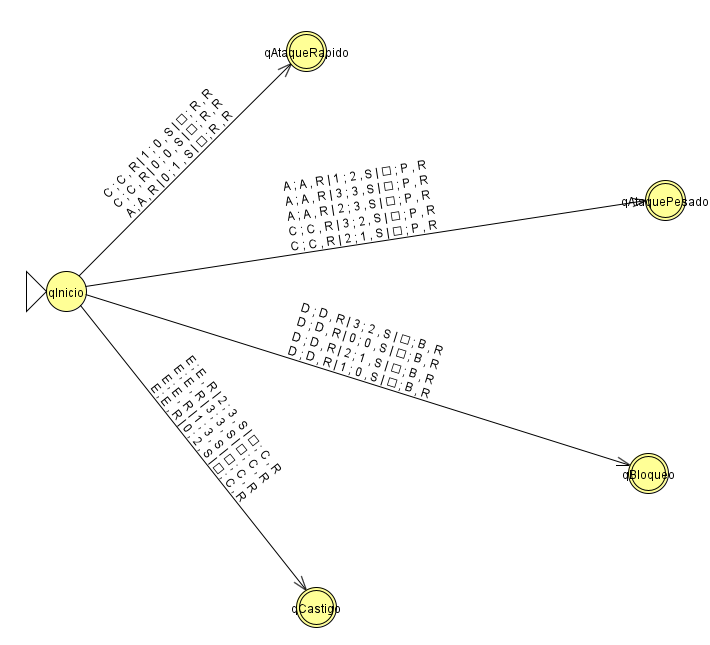
\includegraphics[width=\columnwidth]{maquina_turing.png}
\caption{Máquina de Turing de tres cintas del enemigo, construida en JFLAP. Los cinco estados corresponden a la decisión táctica; las etiquetas de cada arco indican, por cinta, el símbolo leído, el escrito y el movimiento del cabezal.}
\label{fig:maquina}
\end{figure}

\FloatBarrier

La estructura de la figura es la de la definición de la \cref{sec:maquina}: del estado inicial salen las transiciones que clasifican la acción, y cada estado de decisión registra en la tercera cinta el código que el controlador de combate leerá después. Como la máquina es determinista, la figura también lo es: para cada par (estado, símbolos leídos) hay una sola salida, y eso es lo que permite afirmar que dos partidas con la misma secuencia de acciones terminan igual.

Que la máquina exista como dibujo tiene una consecuencia práctica: un diseñador puede revisarla sin leer código. Es el mismo beneficio que un diagrama de estados aporta en la producción de un juego comercial, donde el comportamiento de un personaje se discute sobre el papel antes de programarse \cite{millington2019}.

\subsection{Ejecución del videojuego}
\label{sec:resultado-juego}

La \cref{fig:juego-en-vivo} muestra una partida en ejecución. La arena presenta al jugador y al enemigo, sus barras de vida y la respuesta táctica seleccionada por la máquina; en la parte superior se indican los controles y en la inferior se muestran el golpe activo y el estado de las cintas. Así, la implementación convierte las reglas formales en una interacción visible y jugable.

\begin{figure}[!t]
\centering
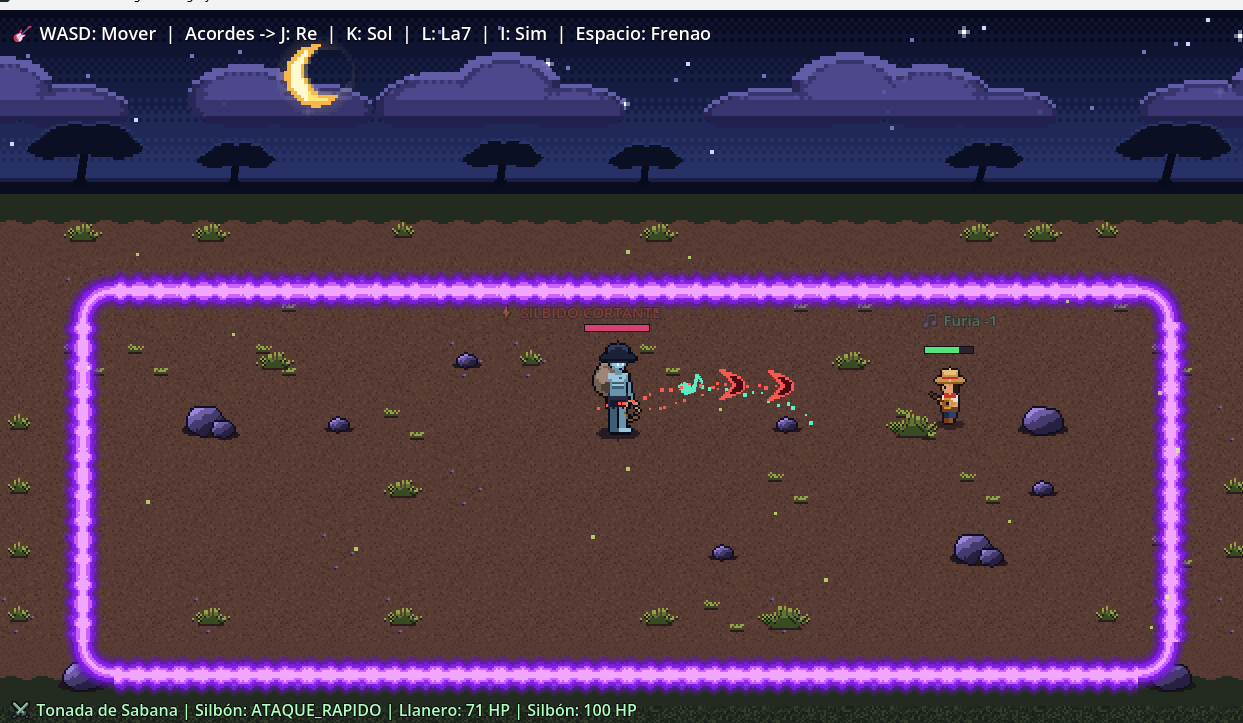
\includegraphics[width=\columnwidth]{resultado_juego.png}
\caption{Ejecución del prototipo de combate. La interfaz muestra la arena, las vidas de ambos personajes, la acción del enemigo y el golpe seleccionado por el jugador.}
\label{fig:juego-en-vivo}
\end{figure}

\FloatBarrier

\subsection{Coherencia del modelo}
\label{sec:coherencia}

La \cref{tab:comportamiento} resume la interacción de las tres piezas ---gramática, máquina y combate--- para cada golpe desde una partida nueva. Los valores son consecuencia directa de las reglas, no una tabla de constantes: \tk{TDDTF} inflige 15 y recibe 10 porque la acción es $A$ y la furia inicial produce ataque rápido; \tk{TSDTF} no inflige daño y anula el contraataque porque la acción $D$ activa el bloqueo y el parry; \tk{TTDF} no pertenece al lenguaje, produce acción \texttt{E}, activa el castigo y recibe 0 de daño directo, pues el código aplica además una inmovilización de $1$ segundo en la presentación.

La tercera repetición consecutiva ilustra el papel de la memoria. Con acciones $A,A,A$, la primera produce ataque rápido, la segunda ataque pesado y la tercera castigo, porque $r'=3$; si la acción repetida es $D$, el castigo se anuncia pero el parry anula el daño. El contrapunteo, por su parte, muestra que la gramática y la máquina son ortogonales: cualquier número de ciclos $\tk{SDT}$ produce el mismo daño de 25 y la misma respuesta enemiga, de modo que la destreza del jugador se mide en la ejecución y no en el poder del golpe.

Esa separación es la que hace el modelo explicable. Un jugador puede describir el sistema con dos frases ---qué combinaciones existen y cómo reacciona el enemigo--- y un diseñador puede modificarlo en dos lugares distintos sin efectos cruzados.

\subsection{Alcance y limitaciones}
\label{sec:alcance}

Los resultados anteriores permiten responder afirmativamente a la pregunta de investigación en lo que respecta al núcleo formal y a la arquitectura: la gramática y la máquina de Turing gobiernan el combate, el contrato es estable y el comportamiento es determinista.

Quedan limitaciones que conviene declarar. La primera es la capa de presentación: el prototipo se concentra en el núcleo, de modo que la experiencia completa ---entrada, audio, HUD de cintas, arena--- todavía no se ha recorrido de principio a fin. La segunda es la clase del lenguaje: como se discutió, $\Lang(G)$ es regular; la gramática y la máquina de Turing son elecciones de especificación y de diseño, no una necesidad expresiva. La tercera es la detección de repetición por categoría de acción y no por canción. La cuarta es la concurrencia: el controlador es único y compartido, de modo que dos clientes simultáneos podrían intercalar turnos; el uso previsto es local y de un jugador, pero una versión multijugador requeriría una sesión por cliente o un bloqueo. La quinta es la ausencia de persistencia: reiniciar el proceso reinicia la partida y las cintas. La sexta es la predictibilidad: al ser determinista, el enemigo puede aprenderse; el reto de diseño es añadir variedad sin perder reproducibilidad, por ejemplo con estados adicionales o con una semilla explícita fuera del núcleo formal.

Una simplificación adicional es que las acciones defensivas y de curación se resuelven por su categoría: el controlador no modela el aturdimiento de Zumbe y Zumbe ni la recuperación de vida de Tonada. La respuesta distingue el golpe, pero el efecto se reduce a ``sin daño'' para las acciones $D$ y $C$. Incorporar esos efectos exigiría ampliar el estado del combate y, probablemente, la máquina de Turing.


\section{Conclusiones y trabajo futuro}
\label{sec:conclusiones}

Este trabajo empezó con una pregunta de aula y terminó mostrando otra cosa: la gramática y la máquina de Turing no son solo contenido evaluable, son infraestructura de producción. En la industria del videojuego esa infraestructura aparece en cuatro frentes.

El primero es el contenido. Las gramáticas generan niveles, misiones, árboles de habilidades y narrativa a partir de reglas; el diseñador deja de enumerar casos y empieza a escribir el espacio de posibilidades \cite{shaker2016}. El contrapunteo de \emph{El Cuatro Llanero} es una versión mínima de esa idea: una regla recursiva produce infinitas cadenas válidas con un daño constante.

El segundo es el lenguaje. Los motores incorporan lenguajes de guion, de configuración y de modificación que se compilan con analizadores generados; sin un reconocedor, el contenido de un diseñador no puede ejecutarse de forma segura \cite{gregory2018,nystrom2014,parr2013}. Un juego que acepta secuencias de un jugador es, en pequeño, el mismo problema: decidir si una entrada pertenece a un lenguaje y qué hacer con ella.

El tercero es el comportamiento. Las máquinas de estado finito siguen siendo el esqueleto de la inteligencia de los personajes, y los árboles de comportamiento se entienden mejor como una generalización de esa idea \cite{millington2019}. La máquina de tres cintas de este trabajo muestra por qué: separar historial, estado interno y decisión hace que el comportamiento sea legible, discutible y modificable.

El cuarto es la reproducibilidad. Un núcleo determinista permite repetir una partida, comparar dos versiones del balance y auditar una queja; esa propiedad, que en un juego comercial se persigue con registros y semillas, aquí es una consecuencia del modelo \cite{gregory2018}. A ello se suma el valor de diseño: cuando la regla formal es la mecánica, el diseñador y el programador trabajan sobre el mismo objeto, y la discusión sobre ``qué se siente justo'' se puede resolver sobre una tabla de transición \cite{salen2004,schell2019}.

La lección principal es que la teoría no necesita un capítulo aparte. Cuando la gramática decide si un ataque existe y la máquina de Turing decide cómo responde el enemigo, el jugador experimenta el modelo formal sin saberlo, y el equipo lo usa como documentación viva. Esa es la utilidad real: no aprobar un examen, sino poder escribir, revisar y cambiar las reglas de un sistema que otras personas van a jugar.

El trabajo futuro tiene cuatro frentes. El primero es completar la capa de presentación: entrada y audio del cuatro, cliente TCP, HUD de las tres cintas, barras de vida, muro espectral y animaciones. El segundo es robustecer la arquitectura: una sesión por cliente, bloqueo del controlador, persistencia del estado y reconexión. El tercero es ampliar el modelo formal: compilar la gramática y comparar el analizador generado con el reconocedor, y explorar una mecánica con estructura anidada que haga estrictamente necesario el poder de una gramática libre de contexto. El cuarto es llevar el modelo a un contexto de producción o de aula y observar cómo lo usan diseñadores y estudiantes, que es la pregunta que este prototipo deja abierta.


\begin{thebibliography}{00}
\bibitem{chomsky1956}
N. Chomsky, ``Three models for the description of language,'' \emph{IRE Transactions on Information Theory}, vol. 2, no. 3, pp. 113--124, 1956.

\bibitem{hopcroft2006}
J. E. Hopcroft, R. Motwani, and J. D. Ullman, \emph{Introduction to Automata Theory, Languages, and Computation}, 3rd ed. Pearson/Addison-Wesley, 2006.

\bibitem{sipser2012}
M. Sipser, \emph{Introduction to the Theory of Computation}, 3rd ed. Cengage Learning, 2012.

\bibitem{scott2015}
M. L. Scott, \emph{Programming Language Pragmatics}, 4th ed. Morgan Kaufmann, 2015.

\bibitem{aho2006}
A. V. Aho, M. S. Lam, R. Sethi, and J. D. Ullman, \emph{Compilers: Principles, Techniques, and Tools}, 2nd ed. Pearson, 2006.

\bibitem{grune2008}
D. Grune and C. J. H. Jacobs, \emph{Parsing Techniques: A Practical Guide}. Springer, 2008.

\bibitem{parr2013}
T. Parr, \emph{The Definitive ANTLR 4 Reference}, 2nd ed. Pragmatic Bookshelf, 2013.

\bibitem{nystrom2014}
R. Nystrom, \emph{Game Programming Patterns}. Genever Benning, 2014.

\bibitem{gregory2018}
J. Gregory, \emph{Game Engine Architecture}, 3rd ed. CRC Press, 2018.

\bibitem{millington2019}
I. Millington, \emph{AI for Games}, 3rd ed. CRC Press, 2019.

\bibitem{shaker2016}
N. Shaker, J. Togelius, and M. J. Nelson, \emph{Procedural Content Generation in Games}. Springer, 2016.

\bibitem{salen2004}
K. Salen and E. Zimmerman, \emph{Rules of Play: Game Design Fundamentals}. MIT Press, 2004.

\bibitem{schell2019}
J. Schell, \emph{The Art of Game Design: A Book of Lenses}, 3rd ed. CRC Press, 2019.

\bibitem{gee2003}
J. P. Gee, \emph{What Video Games Have to Teach Us About Learning and Literacy}. Palgrave Macmillan, 2003.

\bibitem{rodger2006}
S. H. Rodger and T. W. Finley, \emph{JFLAP: An Interactive Formal Languages and Automata Package}. Jones and Bartlett, 2006.

\bibitem{antlr2026}
ANTLR Project, ``ANTLR 4 documentation,'' 2026. [Online]. Sitio oficial: antlr.org

\bibitem{jsonschema2020}
JSON Schema Organization, ``JSON Schema: A media type for describing JSON documents (Draft 2020-12),'' 2020. [Online]. Sitio oficial: json-schema.org
\end{thebibliography}

\end{document}
